% cpu/overview.tex
% mainfile: ../perfbook.tex
% SPDX-License-Identifier: CC-BY-SA-3.0

\section{Overview}
\label{sec:cpu:Overview}
%
\epigraph{Mechanical Sympathy: Hardware and software working together in
	  harmony.}{\emph{Martin Thompson}}

컴퓨터 시스템의 스펙 시트를 부주의하게 읽는 것은 누군가를 CPU 성능은
Figure~\ref{fig:cpu:CPU Performance at its Best} 에 그려진 것처럼 가장 빠른
사람이 항상 이기는, 깨끗한 운동장에서의 달리기 경주라고 생각하게 만들 수
있습니다.

\iffalse

Careless reading of computer-system specification sheets might lead one
to believe that CPU performance is a footrace on a clear track, as
illustrated in Figure~\ref{fig:cpu:CPU Performance at its Best},
where the race always goes to the swiftest.

\fi

\begin{figure}[htb]
\centering
\resizebox{3in}{!}{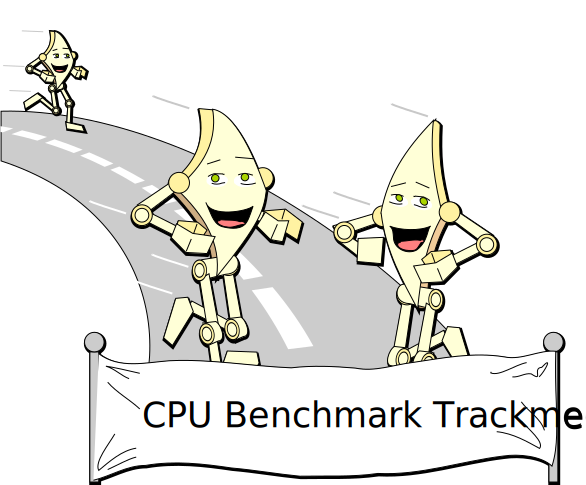
\includegraphics{cartoons/r-2014-CPU-track-meet}}
\caption{CPU Performance at its Best}
\ContributedBy{Figure}{fig:cpu:CPU Performance at its Best}{Melissa Broussard}
\end{figure}

Figure~\ref{fig:cpu:CPU Performance at its Best} 에 그려진 이상적인 경우를
다루는 일부 CPU 국한적 벤치마크들이 존재하지만, 일반적 프로그램은 평범한 달리기
경주보다는 장애물 달리기 경주를 더 닮았습니다.
이는 CPU 의 내부 구조가 지난 수십년간 \IX{Moore의 법칙} 덕에 극적으로 변화했기
때문입니다.
이 변화들을 다음 섹션들에서 설명합니다.

\iffalse

Although there are a few CPU-bound benchmarks that approach the ideal case
shown in Figure~\ref{fig:cpu:CPU Performance at its Best},
the typical program more closely resembles an obstacle course than
a race track.
This is because the internal architecture of CPUs has changed dramatically
over the past few decades, courtesy of \IX{Moore's Law}.
These changes are described in the following sections.

\fi

\subsection{Pipelined CPUs}
\label{sec:cpu:Pipelined CPUs}

\begin{figure}[tb]
\centering
\resizebox{3in}{!}{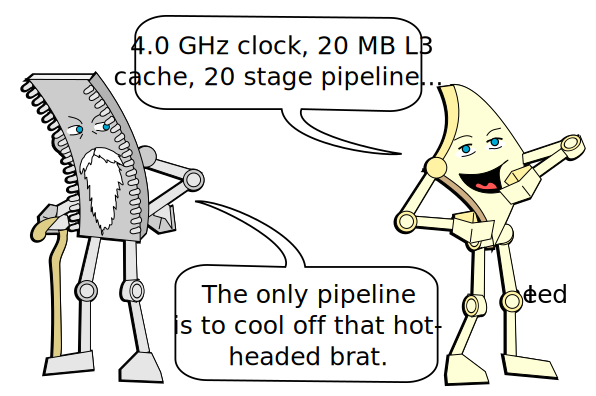
\includegraphics{cartoons/r-2014-Old-man-and-Brat}}
\caption{CPUs Old and New}
\ContributedBy{Figure}{fig:cpu:CPUs Old and New}{Melissa Broussard}
\end{figure}

1980년대에 일반적인 마이크로프로세서는 명령을 (instruction) 가져와 (fetch)
해석하고 (decode) 수행했는데 (execute), 하나의 명령을 완료하는데 일반적으로
\emph{최소} 세개의 클락 사이클을 필요로 했습니다.
반면에, 1990년대 후반과 2000년대의 CPU 는 CPU 를 거치는 명령 과 데이터의 처리
흐름을 최적화 하기 위해 \emph{파이프라인}; \emph{슈퍼스칼라} 기술;
\emph{비순차} 명령과 데이터 처리; \emph{투기적 실행}  기술 등을 사용해 여러
명령을 동시에 수행합니다
일부 코어는 두개 이상의 하드웨어 쓰레드를 갖는데, 이는 \emph{simultaneous
multithreading} (SMT) 또는 \emph{하이퍼쓰레딩} (HT)~\cite{JFennel1973SMT} 이라
불리며, 이 쓰레드 각각은 소프트웨어에게 적어도 기능적 관점에서는 개별 CPU 로
보이게 됩니다.
이런 근대의 하드웨어 기능들은 Figure~\ref{fig:cpu:CPUs Old and New} 에 보여진
것처럼 성능을 상당히 개선할 수 있습니다.

긴 파이프라인을 갖는 CPU 에서 완전한 성능을 이끌어 내는데에는 프로그램의 상당히
예측 가능한 제어 흐름이 필요합니다.
그런 제어 흐름은 예를 들어 거대한 행렬이나 벡터를 가지고 행해지는 계산과 같이
기본적으로 타이트한 반복문을 수행하는 프로그램에서 제공될 수 있습니다.
그럼 CPU 는 이 루프의 끝에서의 브랜치가 거의 모든 경우 취해짐을 제대로 예측할
수 있어서, 파이프라인이 꽉 차게 만들고 CPU 가 완전한 속도로 수행될 수 있게 할
수 있습니다.

\iffalse

In the 1980s, the typical microprocessor fetched an instruction, decoded
it, and executed it, typically taking \emph{at least} three clock cycles
to complete one instruction before even starting the next.
In contrast, the CPU of the late 1990s and of the 2000s execute many
instructions simultaneously, using \emph{pipelines}; \emph{superscalar}
techniques; \emph{out-of-order} instruction and data handling;
\emph{speculative execution}, and
more~\cite{Hennessy2017,Hennessy2011}
in order to optimize the flow of instructions and data through the CPU\@.
Some cores have more than one hardware thread, which is variously called
\emph{simultaneous multithreading} (SMT) or \emph{hyperthreading}
(HT)~\cite{JFennel1973SMT},
each of which appears as
an independent CPU to software, at least from a functional viewpoint.
These modern hardware features can greatly improve performance, as
illustrated by Figure~\ref{fig:cpu:CPUs Old and New}.

Achieving full performance with a CPU having a long pipeline requires
highly predictable control flow through the program.
Suitable control flow can be provided by a program that executes primarily
in tight loops, for example, arithmetic on large matrices or vectors.
The CPU can then correctly predict that the branch at the end of the loop
will be taken in almost all cases,
allowing the pipeline to be kept full and the CPU to execute at full speed.

\fi

\begin{figure}[tb]
\centering
\resizebox{3in}{!}{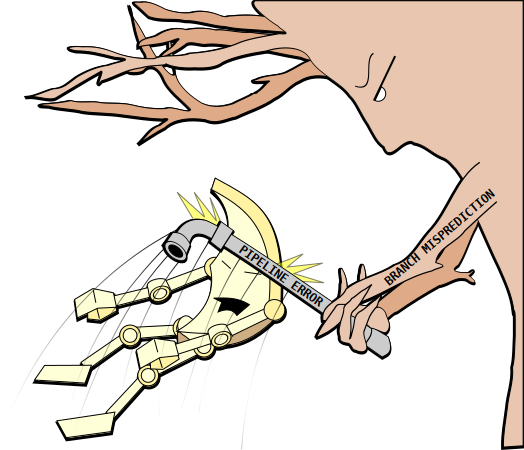
\includegraphics{cartoons/r-2014-branch-error}}
\caption{CPU Meets a Pipeline Flush}
\ContributedBy{Figure}{fig:cpu:CPU Meets a Pipeline Flush}{Melissa Broussard}
\end{figure}

하지만, 브랜치 예측은 항상 쉽지는 않습니다.
예를 들어, 프로그램이 여러 반복문을 포함하며 각각의 반복문은 작은 무작위
횟수만큼 반복되는 경우를 생각해 볼 수 있겠습니다.
또다른 예로, 자주 호출되는 멤버 함수를 갖는 서로 다른 구현체를 갖는 여러 다른
실제 오브젝트를 참조하는 많은 가상 오브젝트를 가져서 결과적으로 많은 수의
포인터 기반 함수 호출을 하게 되는 고전적 객체 지향 프로그램을 생각해 봅시다.
이런 경우, CPU 가 다음 브랜치는 어떻게 될지를 예측하기는 어려우며 불가능할 수도
있습니다.
그럼 CPU 는 그 브랜치가 어느 방향을 향하게 될지 확신할 수 있을 때까지 수행이
진행될 때까지 기다리거나, 추측을 해보고 투기적 수행을 진행해야 합니다.
예측 가능한 제어 흐름을 갖는 프로그램에 대해서는 추측이 매우 잘 동작하지만,
(바이너리 탐색 등의) 예측 불가능한 브랜치들에 대해서는 그 추측이 자주 틀립니다.
잘못된 추측은 그 비용이 비쌀 수 있는데, CPU 는 해당 브랜치를 따라가서
투기적으로 수행된 모든 명령의 결과를 버려야 해서 파이프라인 비우기를 해야 하기
때문입니다.
파이프라인 비우기가 너무 자주 행해지면,
Figure~\ref{fig:cpu:CPU Meets a Pipeline Flush} 에 그려진 것처럼 전체 성능이
무척 감소됩니다.

\iffalse

However, branch prediction is not always so easy.
For example, consider a program with many loops, each of which iterates
a small but random number of times.
For another example, consider an old-school object-oriented program with
many virtual objects that can reference many different real objects, all
with different implementations for frequently invoked member functions,
resulting in many calls through pointers.
In these cases, it is difficult or even
impossible for the CPU to predict where the next branch might lead.
Then either the CPU must stall waiting for execution to proceed far
enough to be certain where that branch leads, or it must guess and
then proceed using speculative execution.
Although guessing works extremely well for programs with predictable
control flow, for unpredictable branches (such as those in binary search)
the guesses will frequently be wrong.
A wrong guess can be expensive because the CPU must discard any
speculatively executed instructions following the corresponding
branch, resulting in a pipeline flush.
If pipeline flushes appear too frequently, they drastically reduce
overall performance, as fancifully depicted in
Figure~\ref{fig:cpu:CPU Meets a Pipeline Flush}.

\fi

\begin{figure}[tb]
\centering
\resizebox{3in}{!}{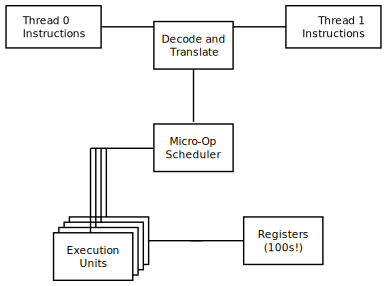
\includegraphics{cpu/microarch}}
\caption{Rough View of Modern Micro-Architecture}
\label{fig:cpu:Rough View of Modern Micro-Architecture}
\end{figure}

이는 갈수록 더 흔해져가는 하이퍼쓰레딩 (또는, 여러분이 그 이름을 선호한다면,
SMT) 에서는 더 나빠지는데, 특히 투기적 수행을 하는 파이프라인 기반의 슈버스칼라
비순차 CPU 에서는 더 그렇습니다.
점점 더 흔해지는 이와 같은 경우, 코어를 공유하는 모든 하드웨어 쓰레드는 이
코어의 레지스터, 캐쉬, 수행 유닛, 등등의 자원을 공유합니다.
명령은 종종 마이크로-오퍼레이션으로 해석되고, 공유된 수행 유닛과 수백개의
하드웨어 레지스터의 사용은 마이크로-오퍼레이션 스케쥴러에 의해 조정됩니다.
그런 두개 쓰레드를 제공하는 코어에 대한 다이어그램이
\cref{fig:cpu:Rough View of Modern Micro-Architecture} 에 그려져 있으며, 더
정확한 (그리고 따라서 더 복잡한) 다이어그램은 교재와 학술 논문에 많이
있습니다.\footnote{
	2010년대 후반 인텔 코어를 위한 예 하나가 여기 있습니다:
	\url{https://en.wikichip.org/wiki/intel/microarchitectures/skylake_(server)}.}
따라서, 한 하드웨어 쓰레드의 수행은 해당 코어를 공유하는 다른 하드웨어 쓰레드의
동작에 의해 자주 방해받을 수 있습니다.

\iffalse

This gets even worse in the increasingly common case of hyperthreading
(or SMT, if you prefer), especially on pipelined superscalar out-of-order
CPU featuring speculative execution.
In this increasingly common case, all the hardware threads sharing
a core also share that core's resources, including registers, cache,
execution units, and so on.
The instructions are often decoded into micro-operations, and use of the
shared execution units and the hundreds of hardware registers is often
coordinated by a micro-operation scheduler.
A rough diagram of such a two-threaded core is shown in
\cref{fig:cpu:Rough View of Modern Micro-Architecture},
and more accurate (and thus more complex) diagrams are available in
textbooks and scholarly papers.\footnote{
	Here is one example for a late-2010s Intel core:
	\url{https://en.wikichip.org/wiki/intel/microarchitectures/skylake_(server)}.}
Therefore, the execution of one hardware thread can and often is perturbed
by the actions of other hardware threads sharing that core.

\fi

오직 하나의 하드웨어 쓰레드만이 활동중이라도 (예를 들어, 단 하나의 쓰레드만
존재하는 고전적 CPU 설계의 경우), 반직관적인 결과는 상당히 흔합니다.
수행 유닛은 겹치는 능력을 가진 경우가 흔해서, CPU 의 수행 유닛 선택이 다음
명령을 위한 해당 수행 유닛에 대한 경쟁이 파이프라인 지연을 야기할 수 있습니다.
이론적으로, 이 경쟁은 회피될 수 있습니다만, 실제로는 CPU 는 천리안 없이도 이
선택을 매우 빨리 해야만 합니다.
특히, 타이트한 반복문에 명령을 추가하는 것은 간혹 수행을 \emph{더 빠르게} 하는
경우도 있습니다.

불행히도, 파이프라인 비우기와 공유 자원 경쟁은 근대의 CPU 가 맞닥뜨리는
장애물의 전부가 아닙니다.
다음 섹션은 메모리 참조에서의 문제를 다룹니다.

\iffalse

Even if only one hardware thread is active (for example, in old-school
CPU designs where there is only one thread), counterintuitive results
are quite common.
Execution units often have overlapping capabilities, so that a CPU's
choice of execution unit can result in pipeline stalls due to contention
for that execution unit from later instructions.
In theory, this contention is avoidable, but in practice CPUs must choose
very quickly and without the benefit of clairvoyance.
In particular, adding an instruction to a tight loop can sometimes
actually cause execution to \emph{speed up}.

Unfortunately, pipeline flushes and shared-resource contention are not
the only hazards in the obstacle course that modern CPUs must run.
The next section covers the hazards of referencing memory.

\fi

\subsection{Memory References}
\label{sec:cpu:Memory References}

1980년대에는 마이크로프로세서가 메모리로부터 값을 읽어오는데 걸리는 시간이
하나의 명령을 수행하는데 걸리는 시간보다 적은 경우가 많았습니다.
최근에는, 마이크로프로세서는 메모리를 액세스하는데 걸리는 시간동안 수백, 또는
심지어 수천개의 명령을 수행할 수도 있습니다.
이 격차는 \IX{무어의 법칙} 이 메모리 반응속도의 감소보다 훨씬 큰 폭으로 CPU
성능을 향상시켰다는 사실 때문입니다.
이는 부분적으로는 메모리 크기 증가 비율 때문이기도 합니다.
예를 들어, 일반적인 1970년대 미니컴퓨터는 4\,KB (그래요, 메가바이트가 아니라
킬로바이트) 메인 메모리를 가졌으며 액세스하는데 단 하나의 사이클이
필요했습니다.\footnote{
	이 단 하나의 사이클이란 게 1.6\emph{마이크로세컨드} 이상의 시간이었음을
	말해두는게 공평하겠습니다.}
오늘날의 CPU 설계자들은 여전히 4\,KB 메모리를 단일 사이클에 액세스 할 수 있도록
할 수도 있는데, 수 GHz 클락 주파수의 시스템에서도 그렇습니다.
그리고 실제로 그런 메모리를 자주 구성합니다만, 그들은 이제 그걸 ``레벨-0 캐쉬''
라 부르며, 그것들은 4\,KB 보다도 상당히 클 수 있습니다.

\iffalse

In the 1980s, it often took less time for a microprocessor to load a value
from memory than it did to execute an instruction.
More recently, microprocessors might execute hundreds or even thousands
of instructions in the time required to access memory.
This disparity is due to the fact that \IX{Moore's Law} has increased CPU
performance at a much greater rate than it has decreased memory latency,
in part due to the rate at which memory sizes have grown.
For example, a typical 1970s minicomputer might have 4\,KB (yes, kilobytes,
not megabytes, let alone gigabytes or terabytes) of main memory, with
single-cycle access.\footnote{
	It is only fair to add that each of these single cycles
	lasted no less than 1.6 \emph{microseconds}.}
Present-day CPU designers still can construct a 4\,KB memory with single-cycle
access, even on systems with multi-GHz clock frequencies.
And in fact they frequently do construct such memories, but they now
call them ``level-0 caches'', plus they can be quite a bit bigger than 4\,KB.

\fi

\begin{figure}[htb]
\centering
\resizebox{3in}{!}{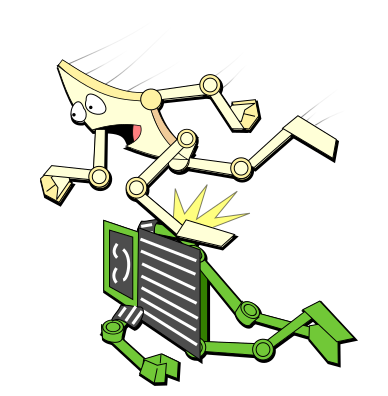
\includegraphics{cartoons/r-2014-memory-reference}}
\caption{CPU Meets a Memory Reference}
\ContributedBy{Figure}{fig:cpu:CPU Meets a Memory Reference}{Melissa Broussard}
\end{figure}

현대 마이크로프로세서에서 찾을 수 있는 대용량 캐쉬가 메모리 접근 반응시간을
해결하는데 상당한 도움이 되지만, 이 캐쉬는 그 반응시간을 숨기는데 성공하기 위해
상당히 예측 가능한 데이터 액세스 패턴을 필요로 합니다.
불행히도, 링크드 리스트를 순회하는 것과 같은 일반적인 오퍼레이션들은 상당히
예측 불가능한 메모리 액세스 패턴을 갖습니다---어쨌건, 그 패턴이 예측
가능하다면, 우리 소프트웨어 측은 포인터를 가지고 고생하지도 않았을 겁니다,
그렇죠?
따라서,
Figure~\ref{fig:cpu:CPU Meets a Memory Reference} 에 보인 것과 같이, 메모리
참조는 현대 CPU 에게 상당한 장애물을 야기합니다.

지금까지 우리는 CPU 가 싱글쓰레드 코드를 수행할 때 마주칠 수 있는 장애물에 대해
생각해 봤습니다.
멀티쓰레딩은 CPU 에 추가적인 장애물을 제공하는데, 다음 섹션들에서 설명합니다.

\iffalse

Although the large caches found on modern microprocessors can do quite
a bit to help combat memory-access latencies,
these caches require highly predictable data-access patterns to
successfully hide those latencies.
Unfortunately, common operations such as traversing a linked list
have extremely unpredictable memory-access patterns---after all,
if the pattern was predictable, us software types would not bother
with the pointers, right?
Therefore, as shown in
Figure~\ref{fig:cpu:CPU Meets a Memory Reference},
memory references often pose severe obstacles to modern CPUs.

Thus far, we have only been considering obstacles that can arise during
a given CPU's execution of single-threaded code.
Multi-threading presents additional obstacles to the CPU, as
described in the following sections.

\fi

\subsection{Atomic Operations}
\label{sec:cpu:Atomic Operations}

그런 장애물 중 하나는 어토믹 오퍼레이션들입니다.
여기서의 문제는 어토믹 오퍼레이션의 개념 자체가 CPU 파이프라인의 한번에 한
조각씩 조립해 나간다는 원칙과 충돌한다는 것입니다.
하드웨어 설계자들 덕분에, 현대의 CPU 는 그런 오퍼레이션들이 실제로는 한번에
한조각씩만 실행됨에도 원자적으로 수행되는 것으로 \emph{보이게} 하는 상당히
영리한 속임수를 사용하는데, 흔히 사용되는 속임수 중 하나는 원자적으로 처리하려
하는 데이터를 포함하고 있는 전체 캐시라인을 인식하고, 해당 캐시라인은 이 어토믹
오퍼레이션을 수행하고 있는 CPU 에게 소유됨을 보장하고, 그런 상태에서만 이
어토믹 오퍼레이션을 진행하는 것입니다.
이 모든 데이터가 이 CPU 에 사적으로 소유되기 때문에, 다른 CPU 들은 CPU 의
한번에 한조각씩 처리하는 파이프라인의 본성에도 불구하고 어토믹 오퍼레이션을
간섭할 수 없습니다.
말할 필요도 없이, 이런 종류의 속임수는 어토믹 오퍼레이션이 올바르게 완료될 수
있도록 하기 위해 이 셋업을 수행하기 위해 파이프라인이 지연되거나 심지어
비워져야만 할 것을 요구할 수도 있습니다.

\iffalse

One such obstacle is atomic operations.
The problem here is that the whole idea of an atomic operation conflicts with
the piece-at-a-time assembly-line operation of a CPU pipeline.
To hardware designers' credit, modern CPUs use a number of extremely clever
tricks to make such operations \emph{look} atomic even though they
are in fact being executed piece-at-a-time,
with one common trick being to identify all the cachelines containing the
data to be atomically operated on,
ensure that these cachelines are owned by the CPU executing the
atomic operation, and only then proceed with the atomic operation
while ensuring that these cachelines remained owned by this CPU\@.
Because all the data is private to this CPU, other CPUs are unable to
interfere with the atomic operation despite the piece-at-a-time nature
of the CPU's pipeline.
Needless to say, this sort of trick can require that
the pipeline must be delayed or even flushed in order to
perform the setup operations that
permit a given atomic operation to complete correctly.

\fi

\begin{figure}[htb]
\centering
\resizebox{3in}{!}{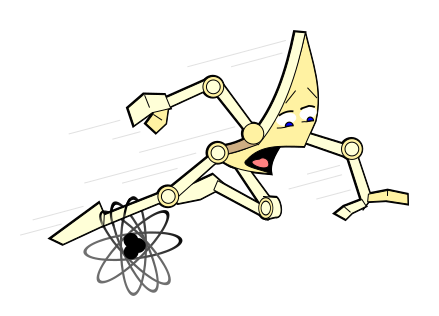
\includegraphics{cartoons/r-2014-Atomic-reference}}
\caption{CPU Meets an Atomic Operation}
\ContributedBy{Figure}{fig:cpu:CPU Meets an Atomic Operation}{Melissa Broussard}
\end{figure}

반면, 비 어토믹 오퍼레이션을 수행할 때에는, CPU 는 캐시라인 소유권을 기다릴
필요 없이 데이터가 나타나자마자 캐시 라인으로부터 값을 읽어들일 수 있으며, 수행
결과를 스토어 버퍼에 저장할 수 있습니다.
가끔 캐쉬 응답시간을 숨길 수 있는 다양한 하드웨어 최적화가 존재하긴 하지만,
이로 인한 성능에의 영향은 너무나도 종종
Figure~\ref{fig:cpu:CPU Meets an Atomic Operation}
에 보인 것과 같습니다.

불행히도, 어토믹 오퍼레이션은 데이터의 단일 원소에만 적용됩니다.
많은 병렬 알고리즘은 순서 규칙이 다수의 데이터 요소의 업데이트 중에도 유지될
것을 필요로 하기 때문에, 대부분의 CPU 는 메모리 배리어를 제공합니다.
이 메모리 배리어는 또한 성능 제약으로 작용하는데, 다음 섹션에서 설명합니다.

\iffalse

In contrast, when executing a non-atomic operation, the CPU can load
values from cachelines as they appear and place the results in the
store buffer, without the need to wait for cacheline ownership.
Although there are a number of hardware optimizations that can sometimes
hide cache latencies, the resulting effect on performance is all too
often as depicted in
Figure~\ref{fig:cpu:CPU Meets an Atomic Operation}.

Unfortunately, atomic operations usually apply only to single elements
of data.
Because many parallel algorithms require that ordering constraints
be maintained between updates of multiple data elements, most CPUs
provide memory barriers.
These memory barriers also serve as performance-sapping obstacles,
as described in the next section.

\fi

\QuickQuiz{

	대체 어떤 기계가 다양한 데이터 원소에 대한 어토믹 오퍼레이션을 허용할
	수 있죠?

	\iffalse

	What types of machines would allow atomic operations on
	multiple data elements?

	\fi

}\QuickQuizAnswer{

	이 질문에 대한 답변 중 하나는 데이터의 여러 원소들을 하나의 기계 단어에
	담을 수 있으며, 그렇게 되면 그것들은 원자적으로 처리될 수 있다는
	것입니다.

	좀 더 시대에 맞춘 답변은 트랜잭셔널 메모리 (transactional memory) 를
	지원하는 기계가 존재한다는 것일
	겁니다~\cite{DBLomet1977SIGSOFT,Knight:1986:AMF:319838.319854,Herlihy93a}.
	2014년 초 기준으로, 여러 주류 시스템이 제한적인 하드웨어 트랜잭셔널
	메모리 구현을 제공하고 있는데,
	Section~\ref{sec:future:Hardware Transactional Memory} 에서 좀 더
	자세한 내용을 다룹니다.
	소프트웨어 트랜잭셔널 메모리의 적용성에 대해선 여전히 평가가
	유보적인데~\cite{McKenney2007PLOSTM,DonaldEPorter2007TRANSACT,
	ChistopherJRossbach2007a,CalinCascaval2008tmtoy,
	AleksandarDragovejic2011STMnotToy,AlexanderMatveev2012PessimisticTM},
	Section~\ref{sec:future:Transactional Memory} 에서 다루겠습니다.

	\iffalse

	One answer to this question is that it is often possible to
	pack multiple elements of data into a single machine word,
	which can then be manipulated atomically.

	A more trendy answer would be machines supporting transactional
	memory~\cite{DBLomet1977SIGSOFT,Knight:1986:AMF:319838.319854,Herlihy93a}.
	By early 2014, several mainstream systems provided limited
	hardware transactional memory implementations, which is covered
	in more detail in
	Section~\ref{sec:future:Hardware Transactional Memory}.
	The jury is still out on the applicability of software transactional
	memory~\cite{McKenney2007PLOSTM,DonaldEPorter2007TRANSACT,
	ChistopherJRossbach2007a,CalinCascaval2008tmtoy,
	AleksandarDragovejic2011STMnotToy,AlexanderMatveev2012PessimisticTM},
	which is covered in Section~\ref{sec:future:Transactional Memory}.

	\fi

}\QuickQuizEnd

\subsection{Memory Barriers}
\label{sec:cpu:Memory Barriers}

Memory barriers will be considered in more detail in
Chapter~\ref{chp:Advanced Synchronization: Memory Ordering} and
Appendix~\ref{chp:app:whymb:Why Memory Barriers?}.
In the meantime, consider the following simple lock-based critical
section:

\begin{VerbatimN}
spin_lock(&mylock);
a = a + 1;
spin_unlock(&mylock);
\end{VerbatimN}

\begin{figure}[tb]
\centering
\resizebox{3in}{!}{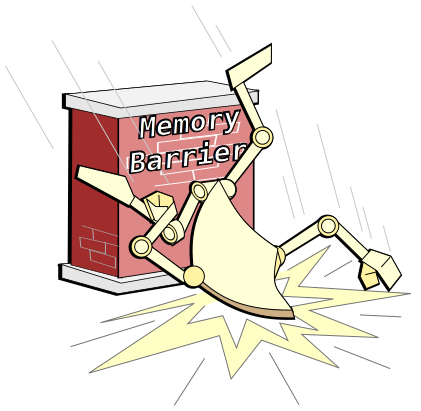
\includegraphics{cartoons/r-2014-Memory-barrier}}
\caption{CPU Meets a Memory Barrier}
\ContributedBy{Figure}{fig:cpu:CPU Meets a Memory Barrier}{Melissa Broussard}
\end{figure}

If the CPU were not constrained to execute these statements in the
order shown, the effect would be that the variable ``a'' would be
incremented without the protection of ``mylock'', which would certainly
defeat the purpose of acquiring it.
To prevent such destructive reordering, locking primitives contain
either explicit or implicit memory barriers.
Because the whole purpose of these memory barriers is to prevent reorderings
that the CPU would otherwise undertake in order to increase performance,
memory barriers almost always reduce performance, as depicted in
Figure~\ref{fig:cpu:CPU Meets a Memory Barrier}.

As with atomic operations, CPU designers have been working hard to
reduce memory-barrier overhead, and have made substantial progress.

\subsection{Cache Misses}
\label{sec:cpu:Cache Misses}

\begin{figure}[tb]
\centering
\resizebox{3in}{!}{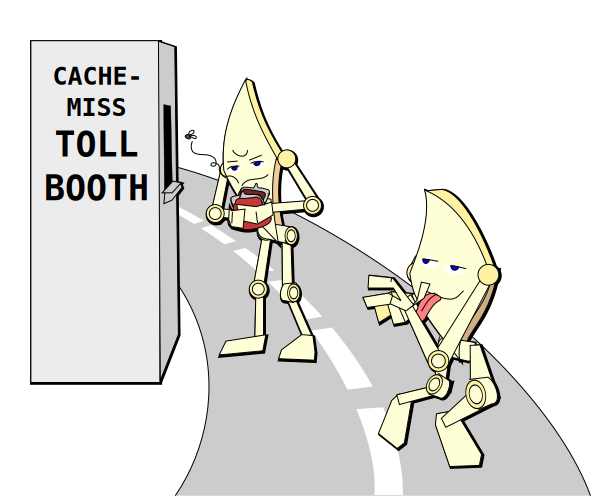
\includegraphics{cartoons/r-2014-CPU-track-meet-cache-miss-toll-booth}}
\caption{CPU Meets a Cache Miss}
\ContributedBy{Figure}{fig:cpu:CPU Meets a Cache Miss}{Melissa Broussard}
\end{figure}

An additional multi-threading obstacle to CPU performance is
the ``cache miss''.
As noted earlier, modern CPUs sport large caches in order to reduce the
performance penalty that would otherwise be incurred due to high memory
latencies.
However, these caches are actually counter-productive for variables that
are frequently shared among CPUs.
This is because when a given CPU wishes to modify the variable, it is
most likely the case that some other CPU has modified it recently.
In this case, the variable will be in that other CPU's cache, but not
in this CPU's cache, which will therefore incur an expensive cache miss
(see Section~\ref{sec:app:whymb:Cache Structure} for more detail).
Such cache misses form a major obstacle to CPU performance, as shown
in Figure~\ref{fig:cpu:CPU Meets a Cache Miss}.

\QuickQuiz{
	So have CPU designers also greatly reduced the overhead of
	cache misses?
}\QuickQuizAnswer{
	Unfortunately, not so much.
	There has been some reduction given constant numbers of CPUs,
	but the finite speed of light and the atomic nature of
	matter limits their ability to reduce cache-miss overhead
	for larger systems.
	Section~\ref{sec:cpu:Hardware Free Lunch?}
	discusses some possible avenues for possible future progress.
}\QuickQuizEnd

\subsection{I/O Operations}
\label{sec:cpu:I/O Operations}

\begin{figure}[tb]
\centering
\resizebox{3in}{!}{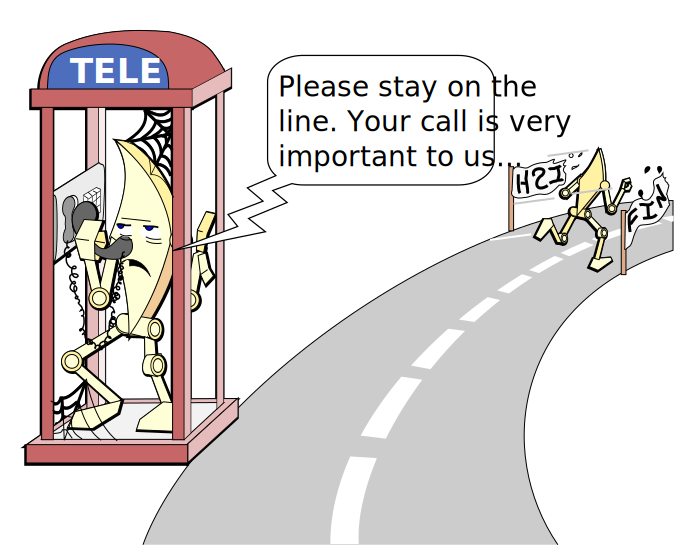
\includegraphics{cartoons/r-2014-CPU-track-meet-phone-booth}}
\caption{CPU Waits for I/O Completion}
\ContributedBy{Figure}{fig:cpu:CPU Waits for I/O Completion}{Melissa Broussard}
\end{figure}

A cache miss can be thought of as a CPU-to-CPU I/O operation, and as
such is one of the cheapest I/O operations available.
I/O operations involving networking, mass storage, or (worse yet) human
beings pose much greater obstacles than the internal obstacles called
out in the prior sections,
as illustrated by
Figure~\ref{fig:cpu:CPU Waits for I/O Completion}.

This is one of the differences between shared-memory and distributed-system
parallelism: shared-memory parallel programs must normally deal with no
obstacle worse than a cache miss, while a distributed parallel program
will typically incur the larger network communication latencies.
In both cases, the relevant latencies can be thought of as a cost of
communication---a cost that would be absent in a sequential program.
Therefore, the ratio between the overhead of the communication to
that of the actual work being performed is a key design parameter.
A major goal of parallel hardware design is to reduce this ratio as
needed to achieve the relevant performance and scalability goals.
In turn, as will be seen in
Chapter~\ref{cha:Partitioning and Synchronization Design},
a major goal of parallel software design is to reduce the
frequency of expensive operations like communications cache misses.

Of course, it is one thing to say that a given operation is an obstacle,
and quite another to show that the operation is a \emph{significant}
obstacle.
This distinction is discussed in the following sections.
